\subsection{Visualización}

La empresa requirió que se mostrara en una interfaz gráfica un brazo en 2D controlado con los ángulos calculados de la cinemática inversa.

Para desarrollar la aplicación, se utilizó el framework Qt, en el cual se implementaron las etapas de Sensado y Localización en C++. La interfaz se implementó en QML, un lenguaje declarativo que facilitó el desarrollo de la interfaz.

El proceso de lectura de datos del sensor se ejecuta constantemente, lo que puede bloquear los procesos de la interfaz y que ésta deje de responder para el usuario. Para evitar dicho problema, se colocó dicho proceso de lectura de datos en un hilo; éste permite que un subproceso pueda ejecutarse de forma concurrente con otros subprocesos. Para que el hilo de captura de datos pueda comunicar las lecturas a la interfaz, y que éstas puedan ser visualizadas en la interfaz gráfica, se utiliza el paso de mensajes; Qt permite enviar mensajes entre hilos a través de señales. De este modo, también se evitan problemas de concurrencia si ambos hilos intentan acceder a la misma variable donde se almacenan los datos de los sensores.

En la Figura \ref{fig:interfaz} se observa la interfaz con el brazo en 2D; puede notarse que se indica el plano que está siendo visualizado; esto puede ser configurado con el botón arriba a la izquierda. También puede observarse la posición del efector final determinada por la etapa de localización. La gráfica está graduada, de modo que se puede apreciar la precisión del modelo.

\begin{figure}[htb]
	\centering
	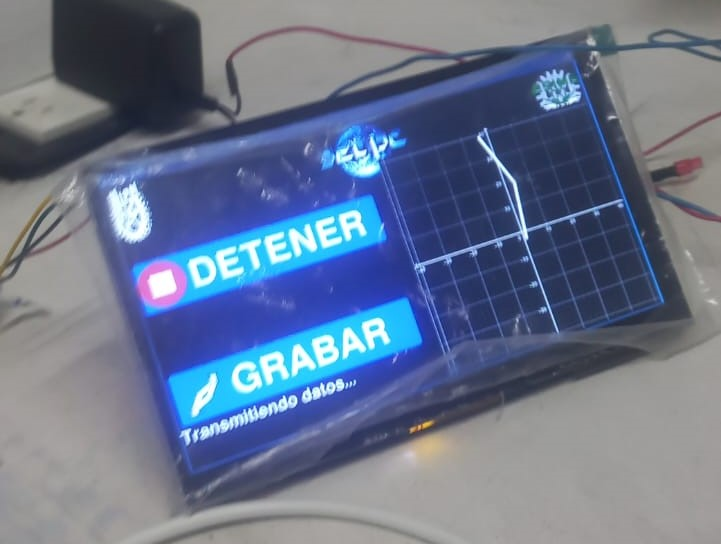
\includegraphics[scale=0.5]{interfaz.jpg}
	\caption{Interfaz gráfica de usuario mostrada en la pantalla táctil de la Raspberry Pi}
	\label{fig:interfaz}
\end{figure}